\documentclass[../main.tex]{subfiles}

\begin{document}

\chapter{Illustration of algorithms}

This appendix illustrates the applied encryption and decryption algorithms.
For details about their functionality have a look to \cref{chap:design}.

\section{Encryption algorithm}
\label{app:encryption}
\begin{figure}[h]
    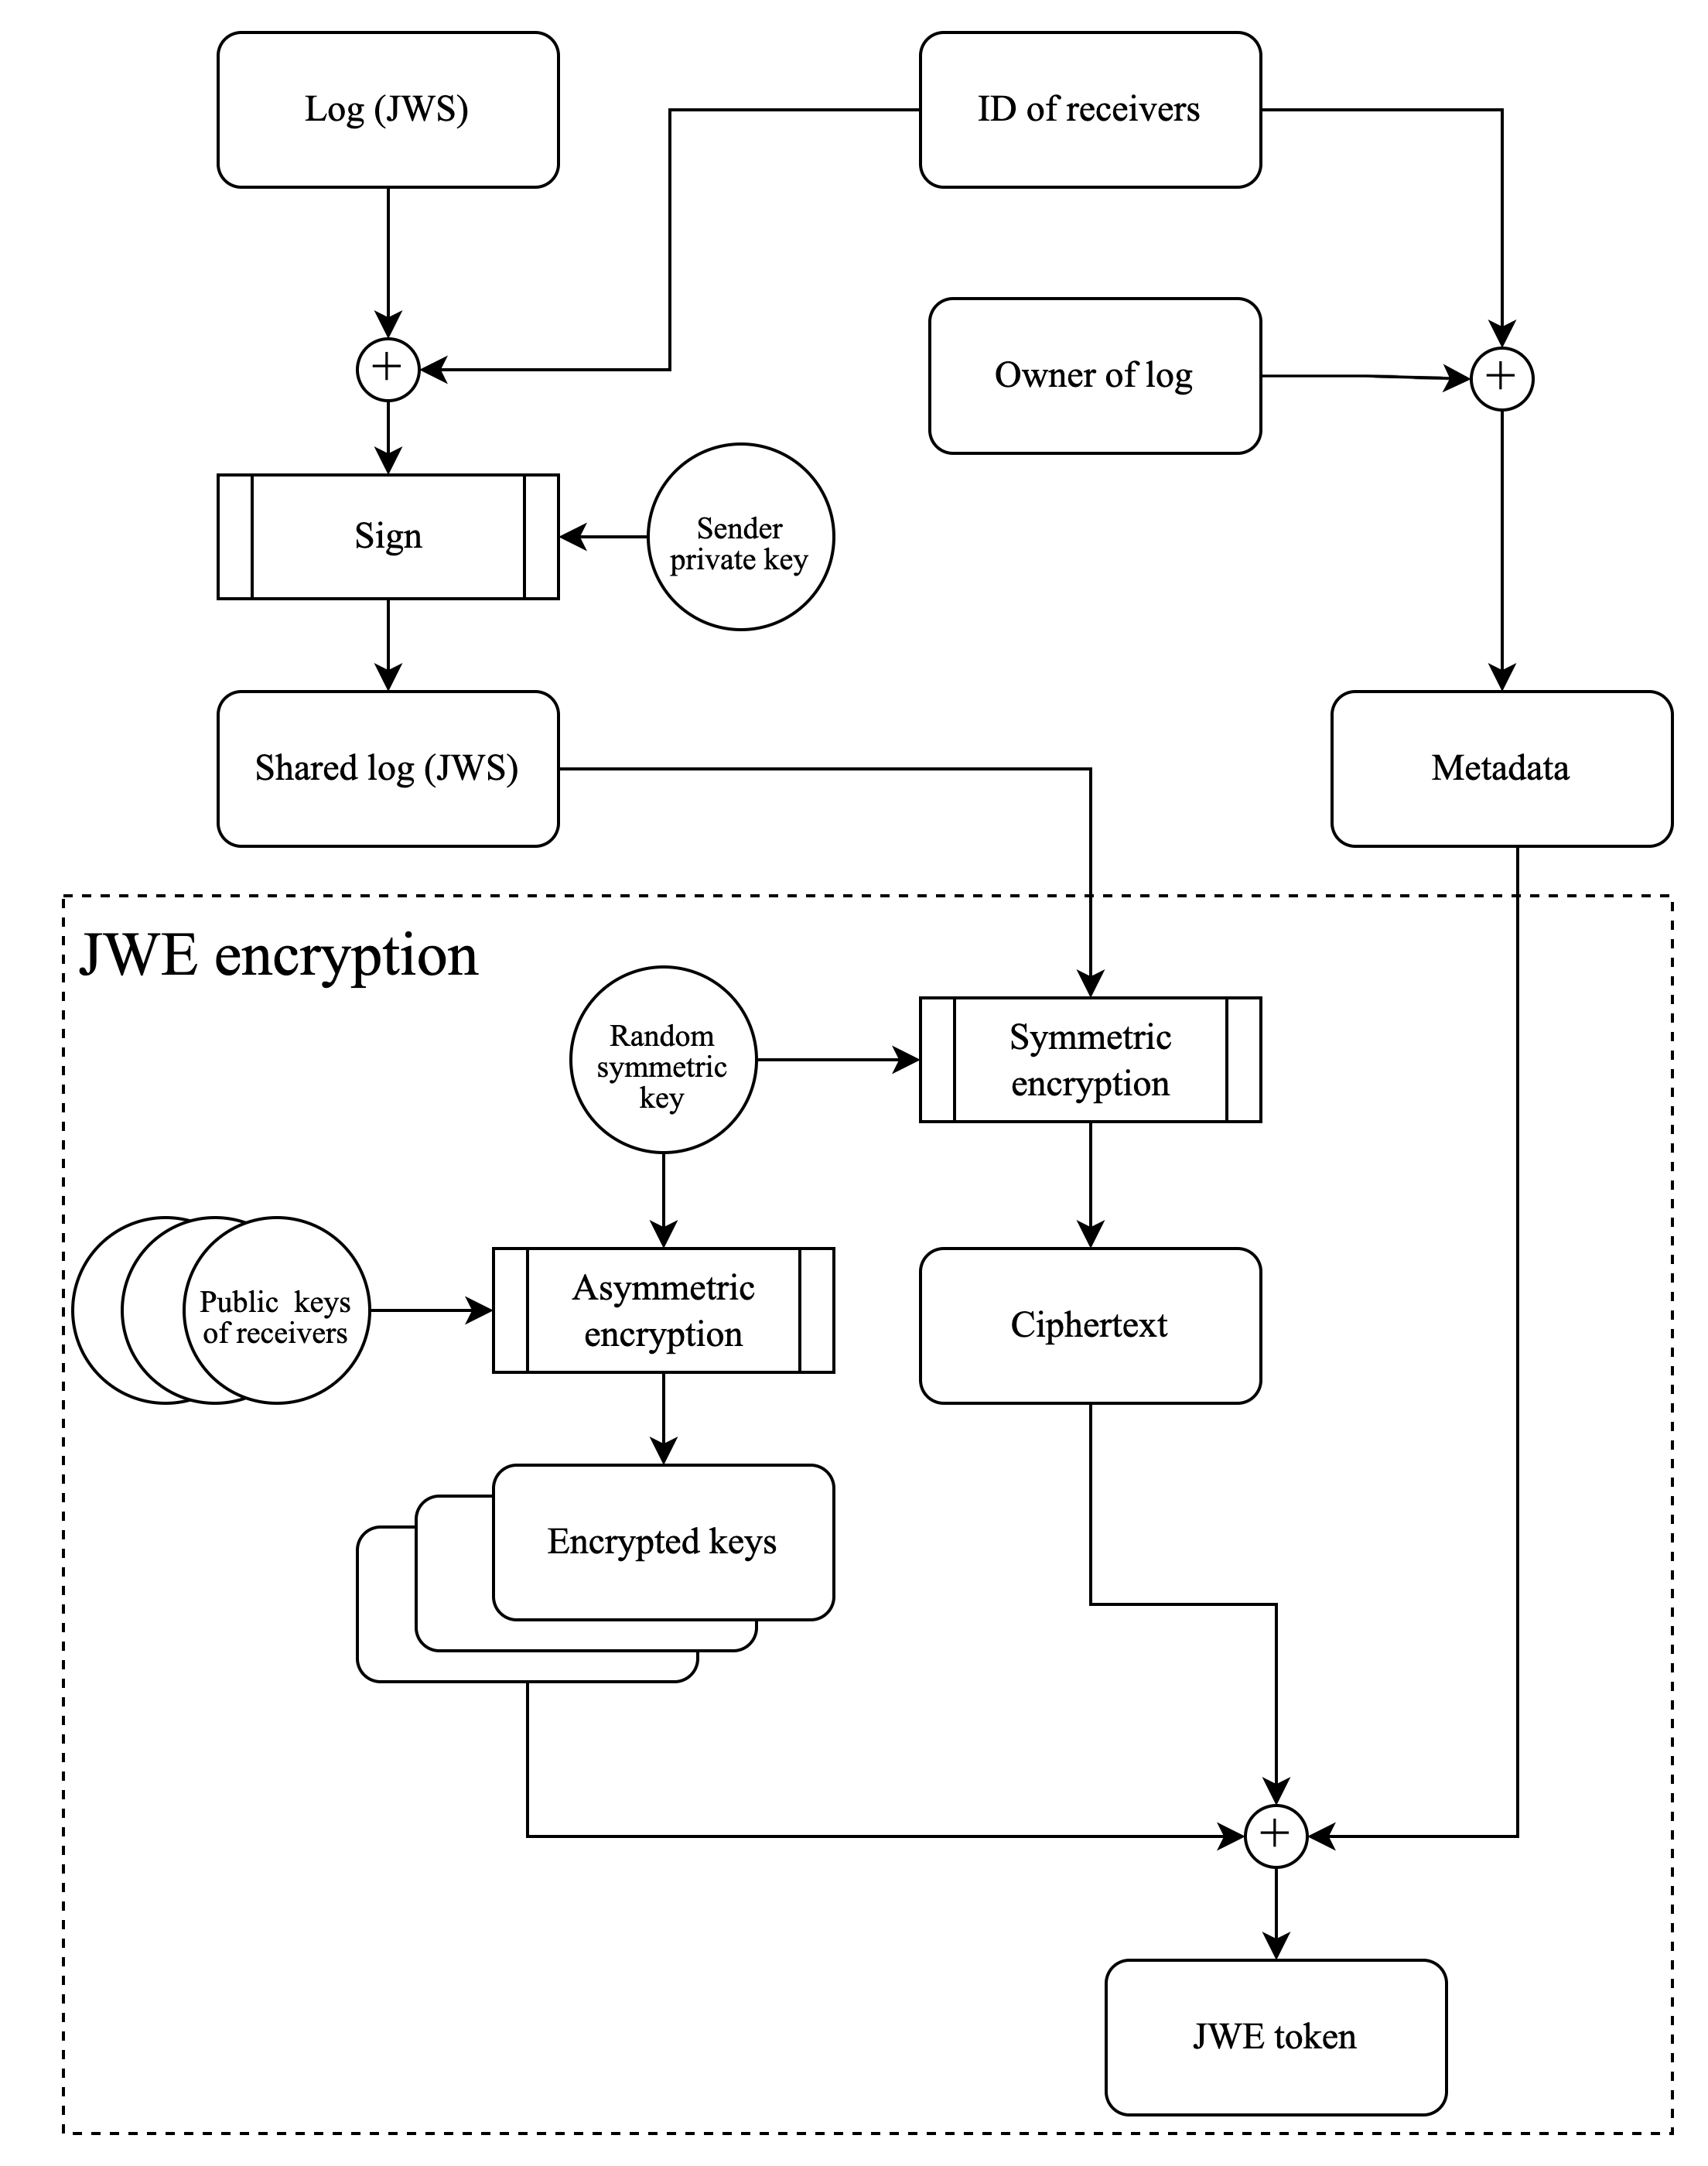
\includegraphics[scale=0.158]{../img/05/encrypt_logs.png}
    \centering
    \caption[Encryption algorithm]{The encryption algorithm takes a signed log and a set of receivers as input. It returns a JWE-token which can only be decrypted by the specified set of users.}
    \label{app:encryption_algo}
\end{figure}
\newpage
\section{Decryption algorithm}
\label{app:decryption}
\begin{figure}[h]
    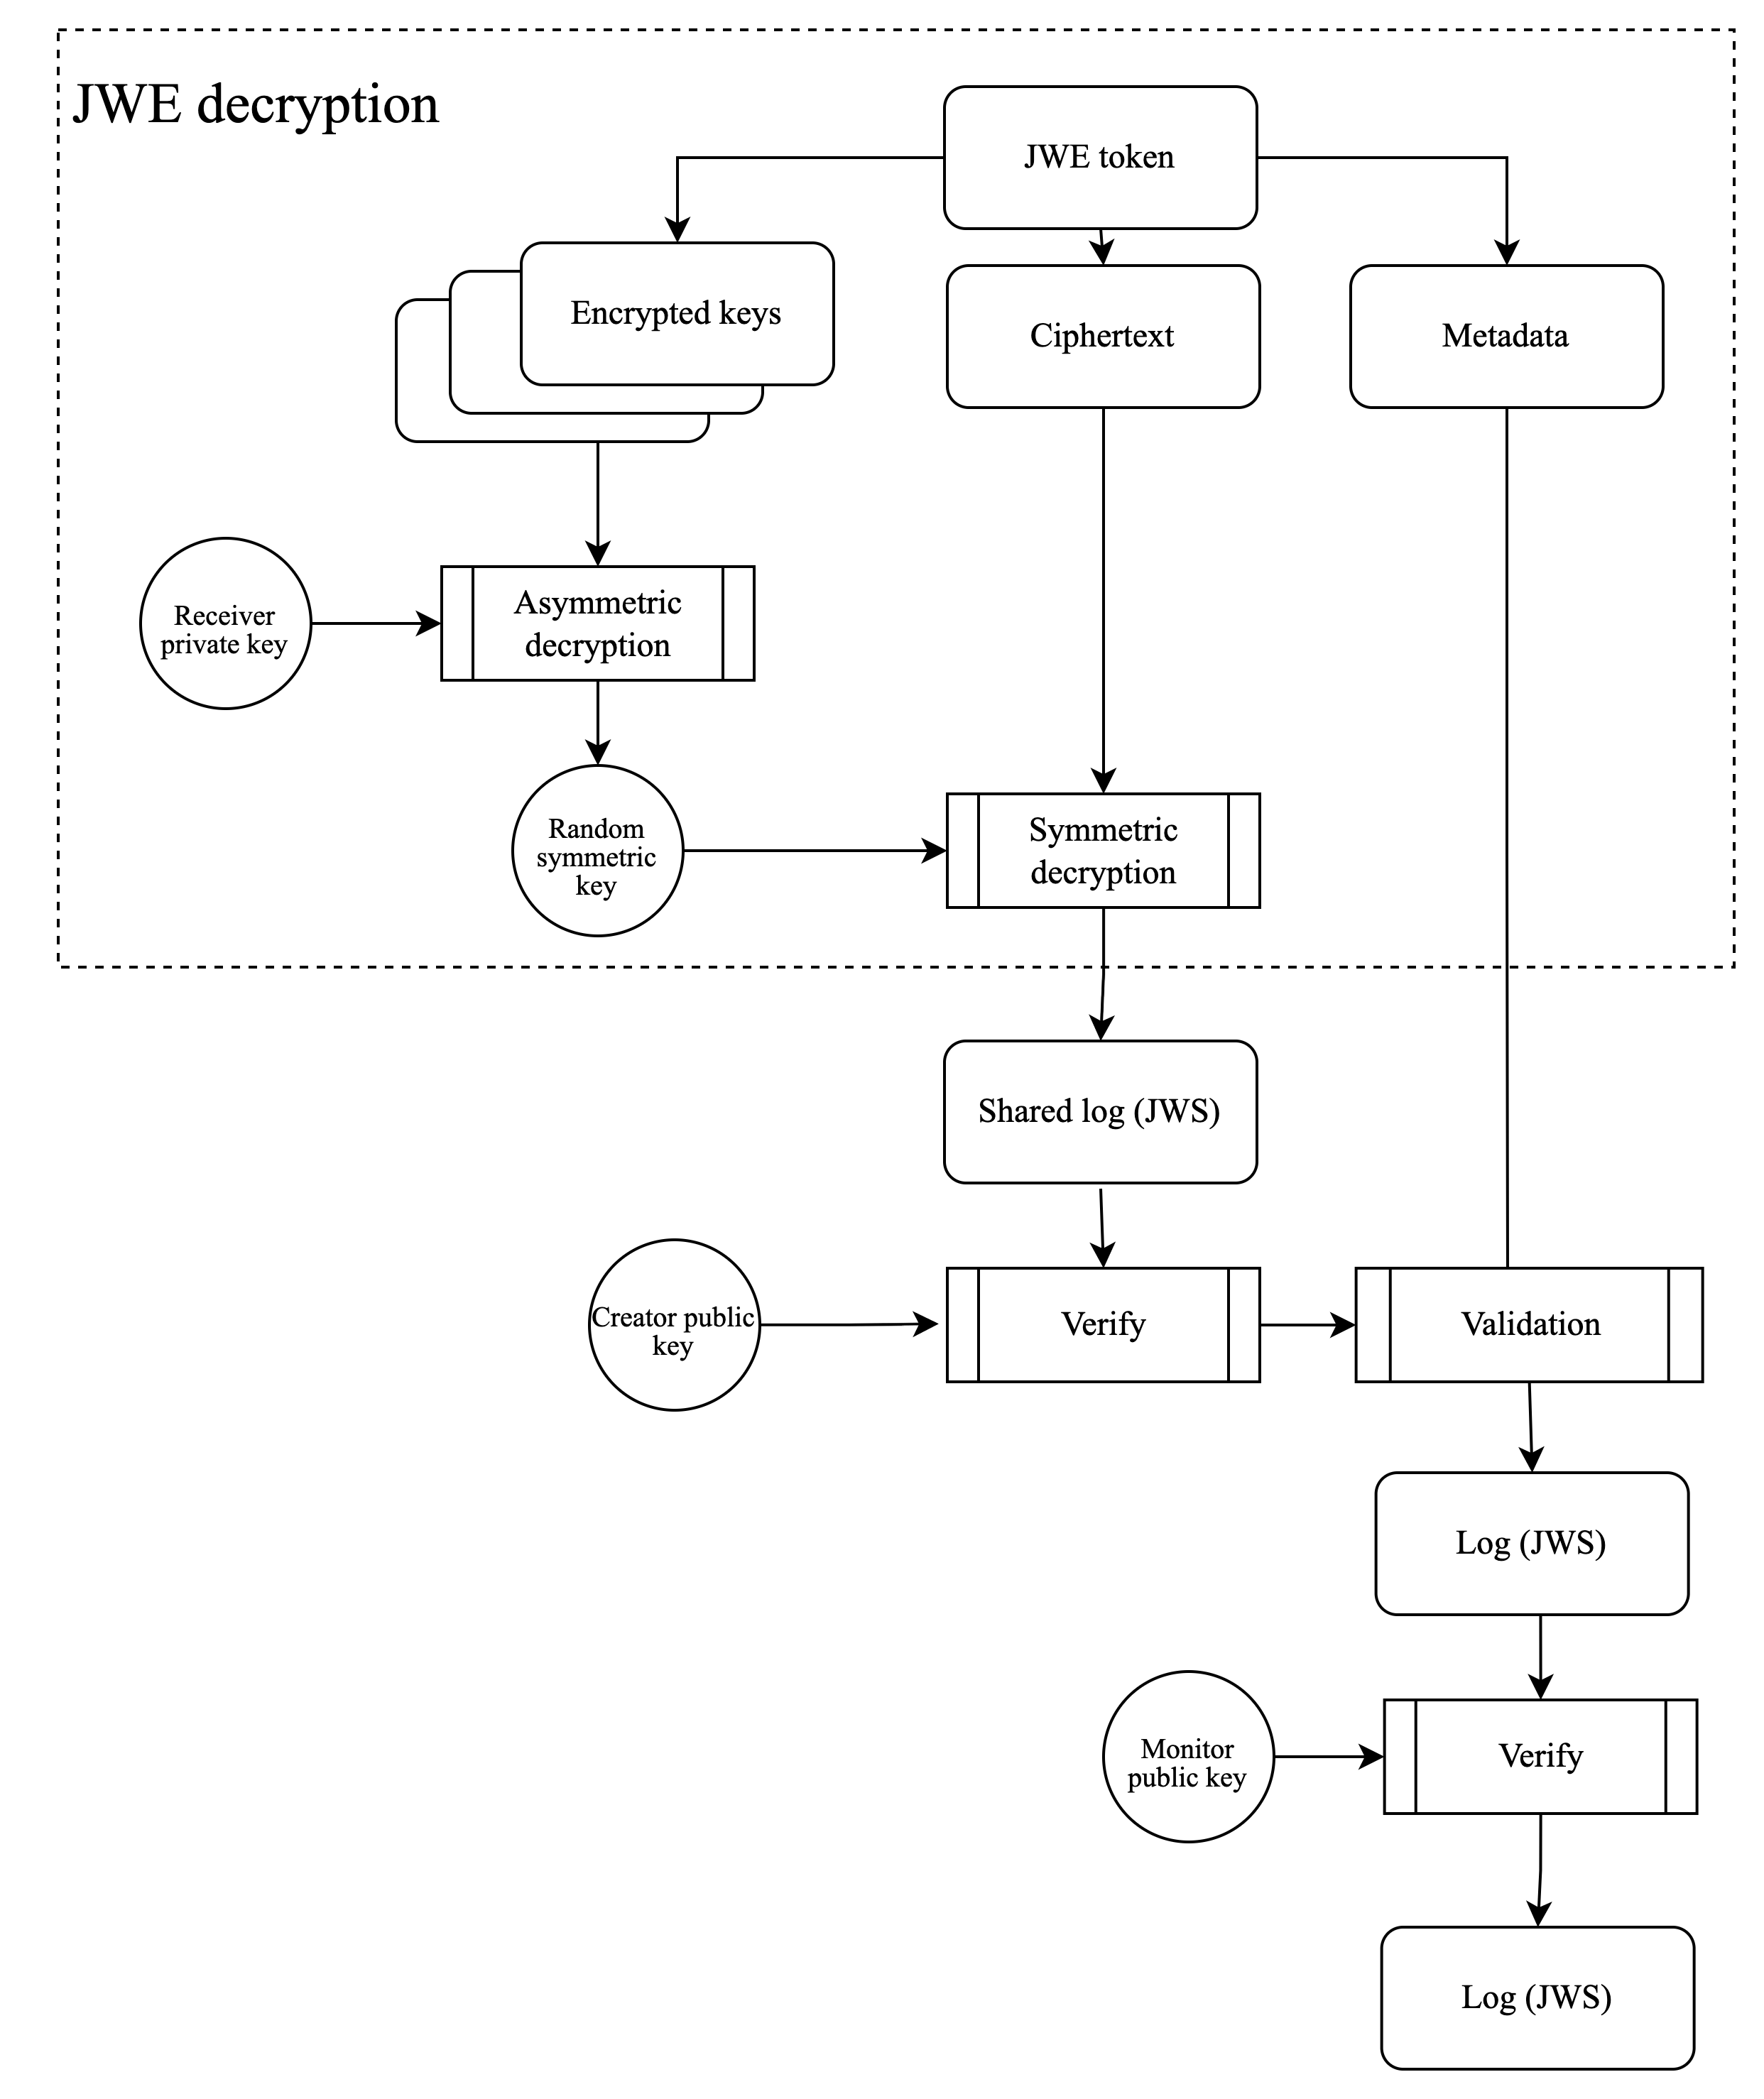
\includegraphics[scale=0.153]{../img/05/decrypt_logs.png}
    \centering
    \caption[Decryption algorithm]{The decryption algorithm takes a JWE token and a private decryption key as input. It returns the decrypted log if the user is allowed to decrypt.}
    \label{app:decryption_algo}
\end{figure}

\chapter{Screenshots Clotilde UI}

This appendix contains screenshots of the implemented features in the \emph{Clotilde UI}.

\label{app:screenshots}
\begin{figure}[h!]
    \fbox{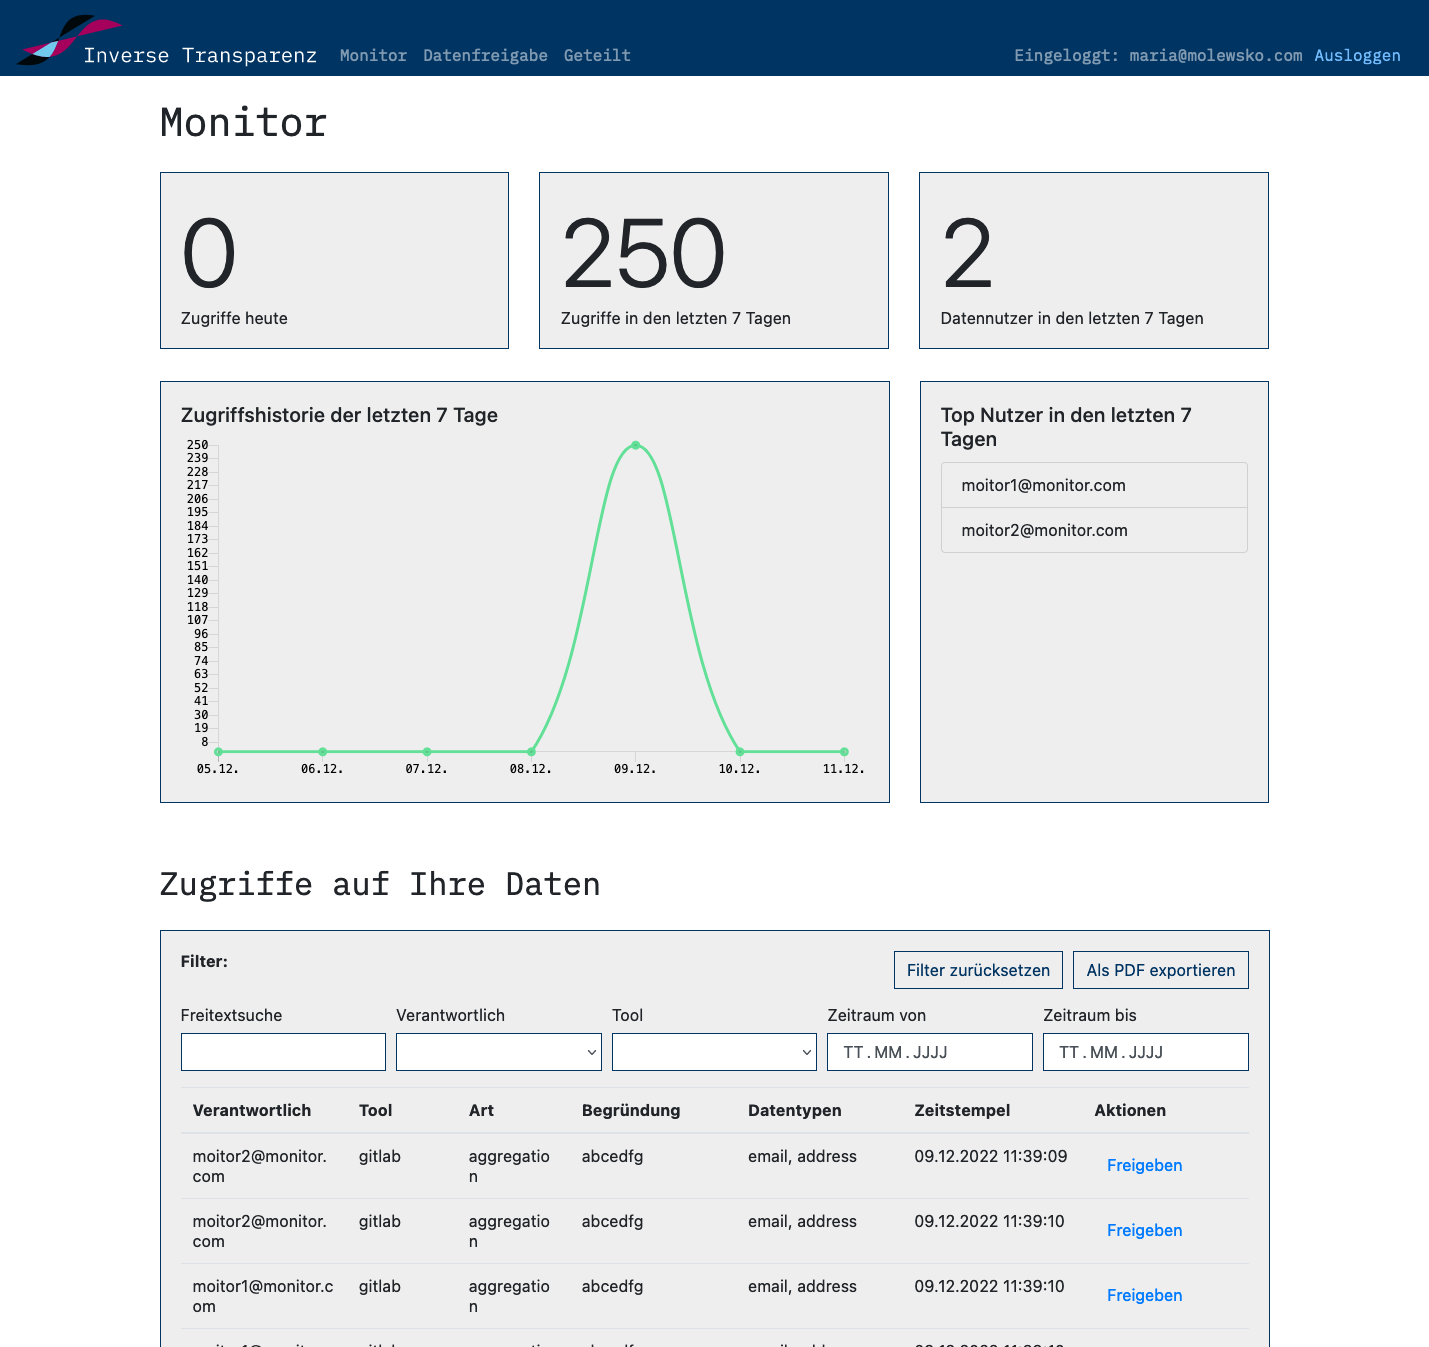
\includegraphics[scale=0.3]{../img/06/clotilde_overview.png}}
    \centering
    \caption[Clotilde UI: Overview]{
        The updated overview page of the Clotilde UI. 
        All logs are visualized as before. 
        The user can share or revoke access to a log by clicking on the corresponding button in the table.}
    \label{app:clotilde-overview}
\end{figure}
\newpage
\begin{figure}[h!]
   \fbox{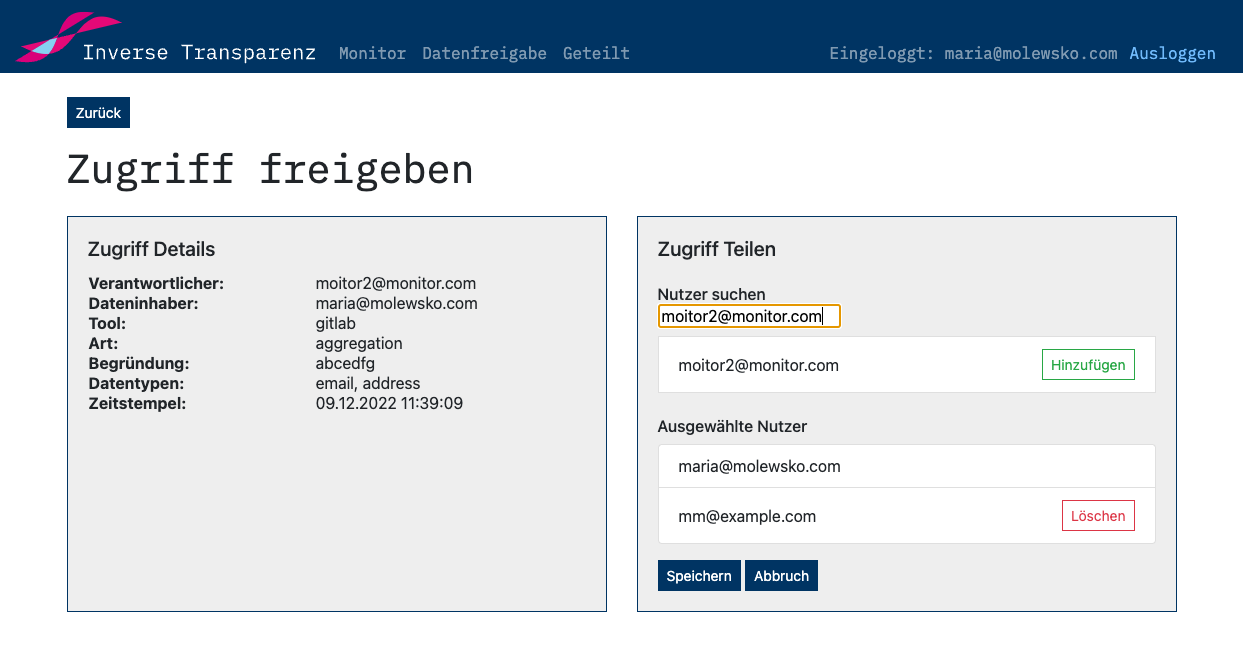
\includegraphics[scale=0.35]{../img/06/clotilde_share.png}}
    \centering
    \caption[Clotilde UI: Share and revoke access]{
        This view allows the user to share or revoke access to a log. 
        On the left-hand side, the details of the log are displayed. 
        On the right-hand side, the user can search for other users in the system. 
        If a user is found, it can be added to the set of recipients. 
        The access to certain users can be revoked by removing them from the list of recipients.}
    \label{app:clotilde-share}
\end{figure}

\begin{figure}[h!]
    \fbox{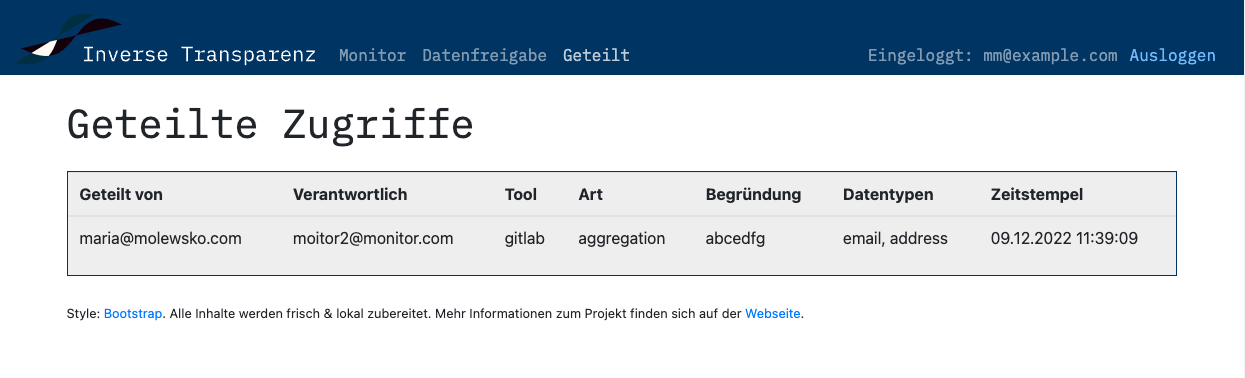
\includegraphics[scale=0.35]{../img/06/clotilde_shared.png}}
    \centering
    \caption[Clotilde Ui: Shared logs]{
        This view lists all logs that are shared with the logged-in users.
        It is realized as additional section within the menu.
    }
    \label{app:clotilde-shared}
\end{figure}

\end{document}
